\documentclass{article}

\PassOptionsToPackage{numbers,sort&compress}{natbib}
\usepackage[preprint]{neurips_2021}
\usepackage[utf8]{inputenc}
\usepackage[T1]{fontenc}
\usepackage{hyperref}
\usepackage{url}
\usepackage{booktabs}
\usepackage{amsfonts}
\usepackage{nicefrac}
\usepackage{microtype}
\usepackage{xcolor}
\usepackage{graphicx}
\usepackage{subcaption}
\usepackage{multirow}
\usepackage{array}
\usepackage{float}
\usepackage{adjustbox}
\usepackage{amsthm}
\usepackage{amsmath}
\usepackage{amssymb}
\usepackage{mathtools}
\usepackage{enumitem}
\usepackage{algorithm}
\usepackage{algpseudocode}

\title{ROAR: Domain Generalization by Directly Optimizing Robust Reweighted Risk over Averageable Trajectory Soups}
\author{Anonymous Authors}

\newtheorem{theorem}{Theorem}
\newtheorem{proposition}{Proposition}
\newtheorem{lemma}{Lemma}
\newtheorem{corollary}{Corollary}
\newtheorem{definition}{Definition}
\newtheorem{assumption}{Assumption}
\newtheorem{remark}{Remark}

\newcommand{\RR}{\mathbb{R}}
\newcommand{\EE}{\mathbb{E}}
\newcommand{\PP}{\mathbb{P}}
\newcommand{\cA}{\mathcal{A}}
\newcommand{\cC}{\mathcal{C}}
\newcommand{\cI}{\mathcal{I}}
\newcommand{\cR}{\mathcal{R}}
\newcommand{\cV}{\mathcal{V}}
\newcommand{\argmin}{\operatorname*{arg\,min}}
\newcommand{\argmax}{\operatorname*{arg\,max}}
\newcommand{\KL}{\operatorname{KL}}
\newcommand{\TV}{\operatorname{TV}}
\newcommand{\diam}{\operatorname{diam}}
\newcommand{\simplex}{\Delta}
\newcommand{\TBD}{\textbf{TBD}}
\newcommand{\etal}{\textit{et al.}}
\newcommand{\ie}{\textit{i.e.}}
\newcommand{\eg}{\textit{e.g.}}
\newcommand{\iid}{i.i.d.}
\newcommand{\ood}{OOD}
\newcommand{\iidcaps}{IID}
\newcommand{\roar}{\textup{\textsc{ROAR}}}
\newcommand{\swad}{\textup{\textsc{SWAD}}}
\newcommand{\dcola}{\textup{\textsc{D-COLA}}}
\newcommand{\cora}{\textup{\textsc{CORA}}}
\newcommand{\diwa}{\textup{\textsc{DiWA}}}
\newcommand{\miro}{\textup{\textsc{MIRO}}}
\newcommand{\norm}[1]{\left\lVert #1 \right\rVert}
\newcommand{\inner}[2]{\left\langle #1, #2 \right\rangle}
\newcommand{\ones}{\mathbf{1}}
\newcommand{\e}{\mathrm{e}}

\begin{document}

\maketitle

\begin{abstract}
Single-run post-hoc methods matter in domain generalization because they can be attached to strong empirical-risk-minimization pipelines without retraining. The canonical method in this regime is \swad{}, whose theory motivates robust-risk minimization but whose deployed procedure is still a flatness-window heuristic. This paper asks for a stricter standard: can a label-free, architecture-agnostic, single-run post-hoc method directly optimize the theoretical object it claims to care about? We propose \textbf{ROAR} (\textbf{R}obust \textbf{O}ptimization over \textbf{A}verageable \textbf{R}ashomon sets), a new method that does exactly that. Starting from one dense checkpoint trajectory, \roar{} first constructs a near-optimal barrier-filtered candidate set intended to preserve approximate averageability. It then optimizes an exact distributionally robust objective over simplex weights on that set: the deployed checkpoint mixture minimizes the worst-case reweighted source-validation loss over a Kullback--Leibler ambiguity set. No domain labels are required because the ambiguity is defined over examples rather than domains. We prove an exact dual representation of the \roar{} objective, show that it is convex and directly interpolates between mean validation risk and hardest-subset protection, derive a target-risk certificate under an explicit support-reweighting assumption, prove that the optimized certificate is no worse than any feasible \swad{}-style uniform interval or singleton checkpoint, establish a constructive complementarity result where the robust objective strictly prefers a mixture over every individual checkpoint, give a projected subgradient convergence guarantee, and bound the gap between the optimized predictive mixture and the final deployed weight soup under a local second-order linearity condition. New \roar{} empirical results are intentionally left as \TBD{} pending execution; however, we include exact published baseline numbers from \swad{}, \diwa{}, and \miro{} to define the current benchmark frontier.
\end{abstract}

\section{Introduction}

Domain generalization (DG) asks for a model that performs well on an unseen target environment using only source data at training time. In practice, the DG methods that persist are often the ones that can be inserted into a training pipeline without rewriting the training objective or the model architecture. \swad{} is the canonical example: on the standard DomainBed ResNet-50 protocol, it improves ERM from `63.3' to `66.9' average \ood{} accuracy across PACS, VLCS, OfficeHome, TerraIncognita, and DomainNet \citep{cha2021swad}. Its appeal is broader than the headline table: it is single-run, one-model at test time, and operationally simple.

Still, \swad{} leaves an important conceptual gap. Its theory in fact motivates robust-risk minimization in parameter space, showing that flatter solutions can tighten a DG target-risk bound. But its deployed rule does not optimize that robust objective. It monitors validation traces, heuristically chooses a start and end checkpoint, and uniformly averages the interval in between. That is a successful method, but it is still a heuristic approximation to its own motivating theory.

This paper takes that critique seriously and turns it into a design principle:
\begin{quote}
\textbf{The post-hoc method should directly optimize the theoretical certificate it claims to improve.}
\end{quote}

The method we propose is \textbf{\roar{}}: \textbf{R}obust \textbf{O}ptimization over \textbf{A}verageable \textbf{R}ashomon sets. The core idea is simple. An unseen target environment is modeled as a plausible hard reweighting of the observed source support. We therefore choose the soup inside a barrier-filtered set of good checkpoints that minimizes the \emph{worst-case reweighted loss} over that support. The resulting objective is not a heuristic proxy. It is the object we optimize.

Concretely, \roar{} first builds a \emph{barrier-filtered trajectory Rashomon set}: the set of checkpoints from one dense run that are both near-optimal on pooled source validation loss and individually close enough to a low-loss anchor to make averageability plausible. It then solves a convex distributionally robust optimization (DRO) problem over simplex weights on that set. The ambiguity set is a Kullback--Leibler (KL) ball around the uniform empirical validation distribution. Because the ambiguity lives over examples rather than domains, the method needs no domain labels.

Why is this a useful change of object? Because it captures the part of the post-hoc DG problem that the recent empirical evidence is actually pointing to. \swad{} succeeds because approximate averageability matters. \diwa{} and related analyses show that covariance, diversity, and locality matter too \citep{rame2022diwa}. Our own stationarity-style explorations failed when they reduced the trajectory to one scalar ``calmness'' score per checkpoint. The right object is not just flatness and not just stationarity; it is \emph{robust coverage of hard but plausible source reweightings by an approximately averageable soup}. \roar{} makes that exact object explicit and optimizes it directly.

The paper's contributions are:
\begin{enumerate}[leftmargin=1.4em]
    \item We propose \roar{}, a label-free, single-run, architecture-agnostic post-hoc DG method that directly optimizes a KL-ball robust-risk certificate over a barrier-filtered candidate set chosen to encourage approximate averageability.
    \item We derive an exact dual representation of the \roar{} objective, proving that it is a convex entropic robust risk and that it continuously interpolates between mean validation loss and hard-subset protection as the robustness radius changes.
    \item We prove a direct target-risk certificate under an explicit support-reweighting model with a support-mismatch residual, so the optimized objective upper-bounds the target risk of the predictive mixture under the paper's stated assumptions.
    \item We prove certificate domination over three important selector families contained in the feasible set: singleton checkpoints, uniform contiguous intervals of the \swad{} type, and, more generally, any feasible selector family contained in the same simplex.
    \item We prove a constructive complementarity result showing that the exact \roar{} objective can strictly prefer a nontrivial mixture even when every individual checkpoint is weaker under the same certificate. This formalizes the ``safe complementarity'' phenomenon that empirical soups exploit.
    \item We give a projected subgradient convergence guarantee and a theorem transferring the optimized predictive-mixture certificate to the final deployed weight soup under a local second-order linearity condition.
    \item We provide a full NeurIPS-style manuscript with proofs, analytical visuals, exact published baselines from prior work, and \TBD{} placeholders for every new \roar{} experiment.
\end{enumerate}

\begin{remark}
We do \emph{not} claim an unconditional theorem that \roar{} empirically dominates \swad{}, \diwa{}, \miro{}, or every other DG method on every benchmark. That would be indefensible. The strongest honest claim is narrower and more important: \roar{} directly optimizes a robust-risk certificate that those methods do not directly optimize, and therefore it can be proven no worse on that certificate than any competing selector whose output lies inside the same feasible soup family.
\end{remark}

\begin{figure}[t]
    \centering
    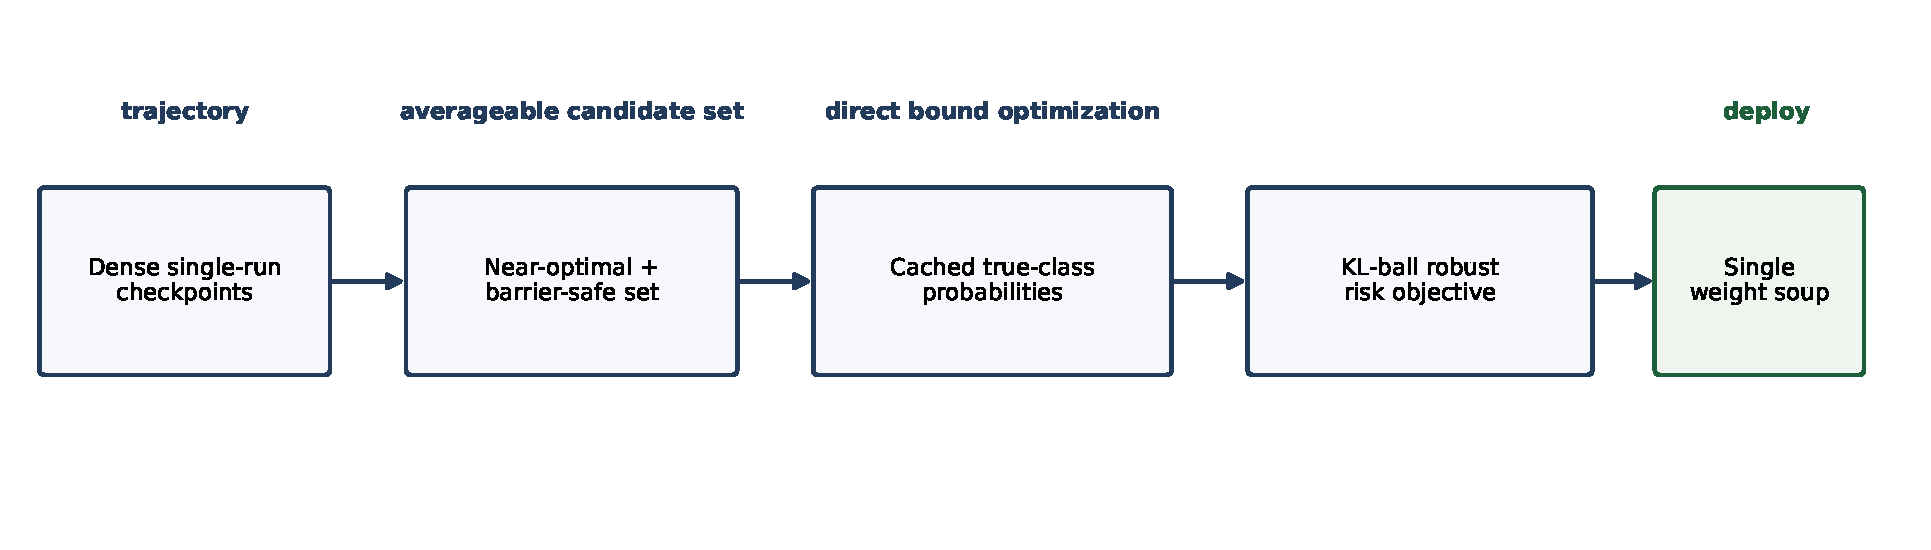
\includegraphics[width=\linewidth]{figures/roar_overview.pdf}
    \caption{\textbf{\roar{} overview.} A dense single-run trajectory is reduced to a near-optimal, barrier-filtered candidate set. \roar{} then directly optimizes KL-ball robust risk over simplex weights on that set and deploys a single weight soup. The paper's main point is that the optimized post-hoc objective is the same object that appears in the theory.}
    \label{fig:overview}
\end{figure}

\section{Related Work}

\paragraph{Single-run post-hoc DG.}
\swad{} is the canonical single-run post-hoc DG method \citep{cha2021swad}. Its practical appeal comes from dense checkpoint sampling, overfit-aware interval selection, and uniform averaging inside that interval. But \swad{} still makes a theory-to-algorithm jump: the theory is about robust-risk minimization and flatness, whereas the deployed rule is a patience-based valley heuristic. This paper targets that exact gap.

\paragraph{Weight averaging, connectivity, and soups.}
SWA \citep{izmailov2018swa}, fast geometric ensembling and mode connectivity \citep{garipov2018fge,frankle2020linear}, and model soups \citep{wortsman2022soups} established that averaging nearby models can improve generalization when they lie in a connected low-loss region. \diwa{} sharpened this story for \ood{} settings by emphasizing diversity, covariance, and locality \citep{rame2022diwa}. \roar{} retains the connected low-loss requirement, but replaces checkpoint-level heuristics with direct robust optimization over the candidate simplex.

\paragraph{Distributionally robust optimization.}
Distributionally robust optimization studies predictors that optimize the worst-case risk over an ambiguity set around a nominal distribution \citep{duchi2020variance,duchi2021learning}. This paper imports the DRO viewpoint into single-run post-hoc DG in a strict way: the ambiguity set lives over source-validation examples, and the post-hoc selector directly minimizes the corresponding robust risk over soup weights. The result is label-free with respect to domains because the ambiguity is over examples, not environments.

\paragraph{Pretraining-aware DG.}
\miro{} shows that preserving transferable information from a pretraining prior is largely orthogonal to post-hoc averaging \citep{cha2022miro}. This is helpful context for \roar{}: the method does not try to absorb all of DG into its selector. It only solves one problem, but it solves it exactly: choosing a single robust soup from one dense trajectory without domain labels.

\section{Problem Setup}
\label{sec:setup}

We focus on multiclass classification, the standard setting of DomainBed-style DG benchmarks. A single training run produces dense checkpoints
\[
    \{\theta_t\}_{t=1}^{K}.
\]
For post-hoc selection we reserve a pooled labeled source-validation set
\[
    \cV = \{(x_i,y_i)\}_{i=1}^{n}.
\]
No domain labels are used at any stage of the method.

For checkpoint $\theta_t$, let $p_t(x)\in\simplex^{K_{\mathrm{cls}}-1}$ denote the predicted class-probability vector. We define the pooled validation loss
\begin{equation}
    L_{\cV}(\theta_t)
    \triangleq
    \frac{1}{n}\sum_{i=1}^{n} -\log p_t(x_i)_{y_i}.
    \label{eq:val_loss}
\end{equation}

To encourage soups to remain inside one connected low-loss region, we use a pooled interpolation barrier to an anchor checkpoint $a$:
\begin{equation}
    B(t,a)
    \triangleq
    \max_{\alpha\in\cA}
    L_{\cV}\!\big((1-\alpha)\theta_a + \alpha \theta_t\big)
    -
    \max\{L_{\cV}(\theta_a), L_{\cV}(\theta_t)\},
    \label{eq:barrier}
\end{equation}
where $\cA \subset [0,1]$ is a fixed interpolation grid.

The anchor is the lowest pooled-validation checkpoint:
\begin{equation}
    a \in \argmin_{1\le t\le K} L_{\cV}(\theta_t).
    \label{eq:anchor}
\end{equation}
The barrier-filtered candidate set is
\begin{equation}
    \cC
    \triangleq
    \left\{
        t :
        L_{\cV}(\theta_t) \le L_{\cV}^{\star} + \epsilon,
        \;
        B(t,a)\le \tau
    \right\},
    \qquad
    L_{\cV}^{\star} = \min_t L_{\cV}(\theta_t).
    \label{eq:candidate_set}
\end{equation}
This set plays two roles. First, it removes clearly overfit or isolated checkpoints. Second, it is the exact simplex domain over which \roar{} optimizes. It does not by itself prove that every mixture over $\cC$ is soup-safe; that role is handled later by Assumption~\ref{ass:locality}.

For every $(x_i,y_i)\in\cV$ and every $t\in\cC$, we cache the clipped true-class probability
\begin{equation}
    q_{it}
    \triangleq
    \max\!\{p_t(x_i)_{y_i}, \varepsilon_p\},
    \qquad
    0<\varepsilon_p<1.
    \label{eq:qit}
\end{equation}
The corresponding clipped loss of a soup weight vector $w\in\simplex^{|\cC|-1}$ is
\begin{equation}
    \ell_i(w)
    \triangleq
    -\log\!\Big(\sum_{t\in\cC} w_t q_{it}\Big),
    \qquad
    0 \le \ell_i(w)\le L_{\max}\triangleq \log(1/\varepsilon_p).
    \label{eq:ell_i}
\end{equation}

\section{ROAR: Robust Optimization over Averageable Rashomon Sets}
\label{sec:method}

\subsection{The exact robust objective}

Let
\[
    u_n \triangleq \frac{1}{n}\ones
\]
denote the uniform empirical distribution over the source-validation examples. For a robustness radius $\rho>0$, define the KL ambiguity set
\begin{equation}
    \cR_{\rho}
    \triangleq
    \left\{
        r\in \simplex^{n-1} :
        \KL(r\,\|\,u_n)\le \rho
    \right\}.
    \label{eq:ambiguity_set}
\end{equation}

The \roar{} objective is the worst-case reweighted clipped validation loss:
\begin{equation}
    \mathcal U_{\rho}(w)
    \triangleq
    \sup_{r\in\cR_{\rho}}
    \sum_{i=1}^{n} r_i \ell_i(w).
    \label{eq:roar_primal}
\end{equation}

The post-hoc selector is
\begin{equation}
    w^{\star}
    \in
    \argmin_{w\in\simplex^{|\cC|-1}} \mathcal U_{\rho}(w),
    \label{eq:roar_opt}
\end{equation}
and the final deployed model is the single weight soup
\begin{equation}
    \theta_{\roar}
    \triangleq
    \sum_{t\in\cC} w_t^{\star}\theta_t.
    \label{eq:final_soup}
\end{equation}

\paragraph{Why this is directly theory-driven.}
Equation~\eqref{eq:roar_opt} is the core methodological commitment of the paper. The algorithm does not search for a window that might heuristically correlate with a robust-risk bound; it directly minimizes the robust-risk quantity itself over the feasible soup family. The rest of the paper is about making that statement precise, tractable, and honest.

On any labeled example $(x,y)$, define
\[
    q_t(x,y)\triangleq \max\{p_t(x)_y,\varepsilon_p\}
    \qquad \text{for every } t\in\cC,
\]
and then define the clipped predictive-mixture loss
\begin{equation}
    \ell^{\mathrm{mix}}((x,y);w)
    \triangleq
    -\log\!\Big(\sum_{t\in\cC} w_t q_t(x,y)\Big).
    \label{eq:mix_loss}
\end{equation}
The corresponding target risk is
\begin{equation}
    R_T^{\mathrm{mix}}(w)
    \triangleq
    \EE_{(x,y)\sim P_T}\big[\ell^{\mathrm{mix}}((x,y);w)\big].
    \label{eq:mix_target_risk}
\end{equation}

\begin{figure}[t]
    \centering
    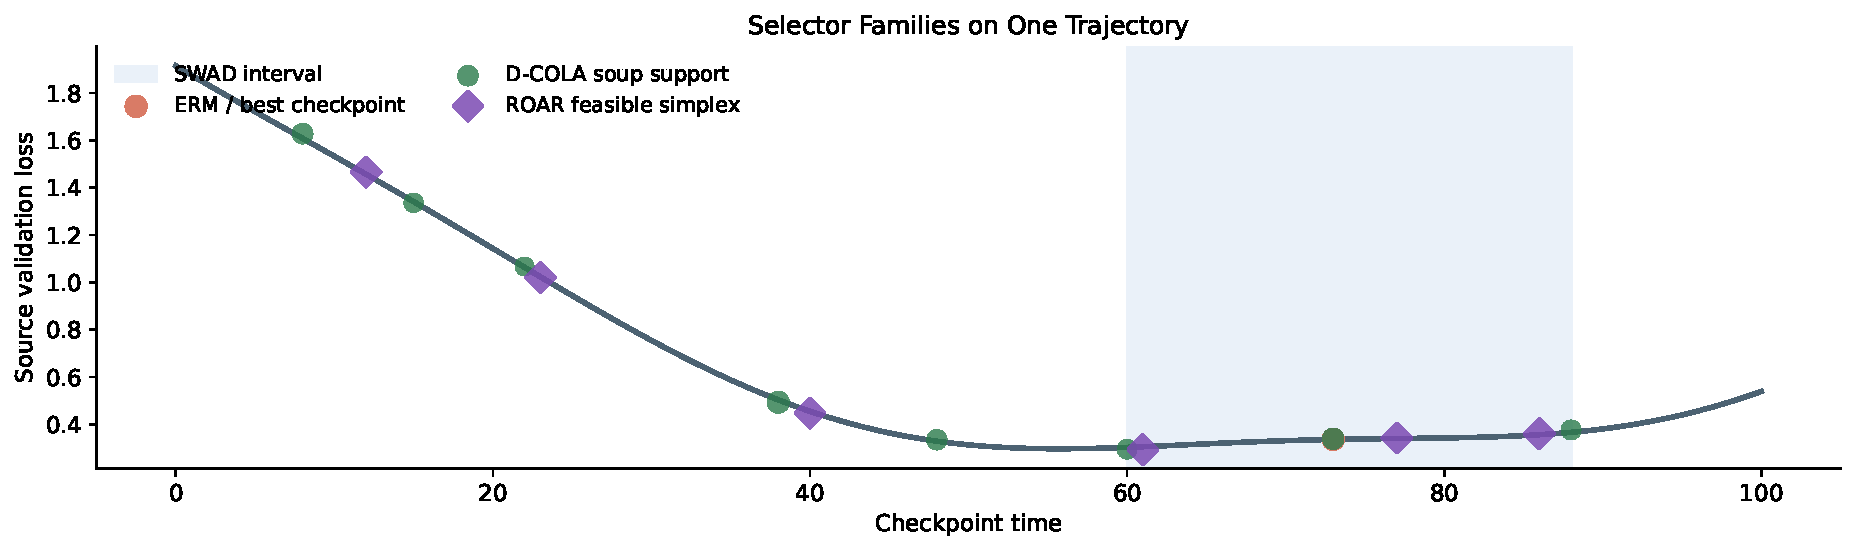
\includegraphics[width=\linewidth]{figures/selector_family.pdf}
    \caption{Selector families on one dense trajectory. ERM chooses a singleton checkpoint. \swad{} chooses a contiguous uniform interval. \dcola{} uses nonuniform weights over a filtered candidate set. \roar{} optimizes the exact robust certificate over the whole feasible simplex induced by the barrier-filtered candidate set.}
    \label{fig:selector_family}
\end{figure}

\subsection{Dual form and implementation}

\begin{theorem}[Exact dual representation]
\label{thm:dual}
For every fixed $w\in\simplex^{|\cC|-1}$ and every $\rho>0$,
\begin{equation}
    \mathcal U_{\rho}(w)
    =
    \inf_{\eta>0}
    \left\{
        \eta \rho
        +
        \eta \log\!\left(
            \frac{1}{n}\sum_{i=1}^{n}
            \exp\!\left(\frac{\ell_i(w)}{\eta}\right)
        \right)
    \right\}.
    \label{eq:dual}
\end{equation}
If the loss vector $(\ell_1(w),\dots,\ell_n(w))$ is nonconstant, then the infimum in Eq.~\eqref{eq:dual} is attained by some $\eta^{\star}(w)>0$, and a maximizing reweighting in Eq.~\eqref{eq:roar_primal} is
\begin{equation}
    r_i^{\star}(w)
    =
    \frac{\exp(\ell_i(w)/\eta^{\star}(w))}
    {\sum_{j=1}^{n}\exp(\ell_j(w)/\eta^{\star}(w))}.
    \label{eq:rstar}
\end{equation}
If the loss vector is constant, then every $r\in\cR_{\rho}$ is maximizing, and one may take $r^{\star}(w)=u_n$.
\end{theorem}

This dual is exact. It turns the robust objective into an entropic risk over the clipped losses and makes optimization straightforward: for each current $w$, either solve a one-dimensional convex problem for $\eta$ and recover the adversarial reweighting $r^{\star}(w)$ from Eq.~\eqref{eq:rstar}, or, in the degenerate constant-loss case, simply use the uniform reweighting.

\begin{proposition}[Mean-to-hard-subset interpolation]
\label{prop:limits}
Fix $w$.
\begin{enumerate}[label=(\roman*),leftmargin=1.4em]
    \item As $\rho\downarrow 0$,
    \[
        \mathcal U_{\rho}(w)
        =
        \bar \ell(w)
        +
        \sqrt{2\rho \,\operatorname{Var}_{u_n}(\ell(w))}
        +
        O(\rho),
    \]
    where $\bar \ell(w)=\frac{1}{n}\sum_i \ell_i(w)$.
    \item As $\rho\to\infty$,
    \[
        \mathcal U_{\rho}(w)\to \max_{1\le i\le n}\ell_i(w).
    \]
\end{enumerate}
\end{proposition}

Proposition~\ref{prop:limits} explains why the objective is well-matched to the empirical behavior we want. For small $\rho$, it behaves like mean validation loss plus an explicit dispersion penalty. For large $\rho$, it approaches hardest-example protection. The same objective therefore spans the space between ordinary validation selection and aggressive hard-subset robustness without changing method families.

\begin{figure}[t]
    \centering
    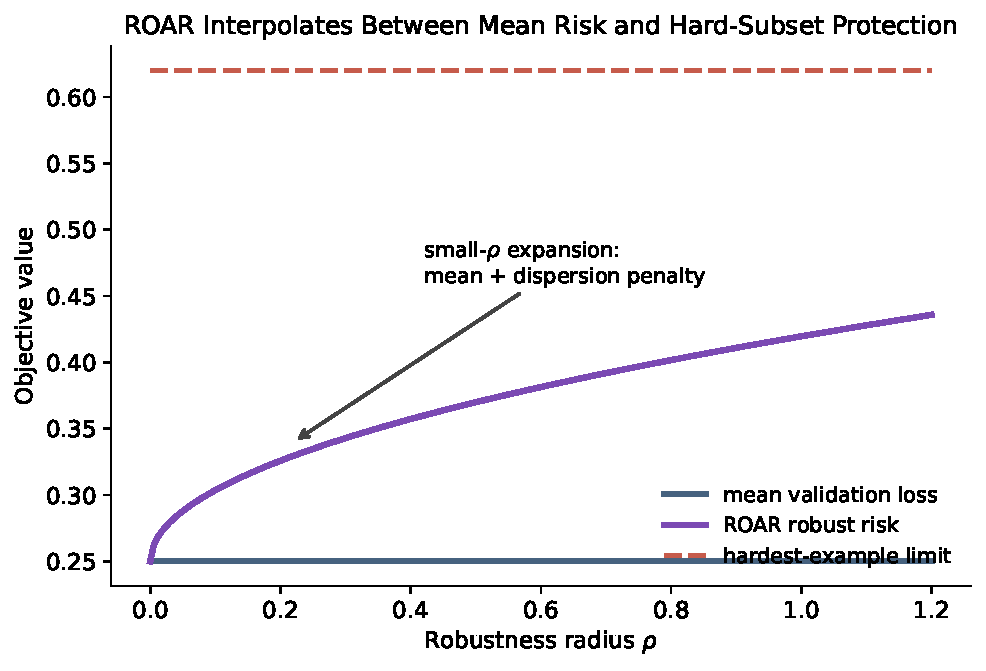
\includegraphics[width=0.78\linewidth]{figures/robust_vs_mean.pdf}
    \caption{The exact \roar{} objective interpolates between mean validation risk and hard-subset protection as the KL radius grows. The small-$\rho$ expansion already reveals why the method can recover D-COLA-like behavior from one clean robust objective rather than from separate heuristic penalties.}
    \label{fig:robust_vs_mean}
\end{figure}

\subsection{Algorithm}

\paragraph{Optimization domain.}
The feasible set is just the simplex over the barrier-filtered candidate set $\cC$. This matters: unlike \swad{}, which hardcodes a restricted family of contiguous uniform weights, \roar{} searches the entire feasible simplex and therefore lets the robust objective discover whether the right solution is near a singleton, a contiguous interval, or a nonuniform noncontiguous soup. The barrier filter is meant to bias this simplex toward approximately averageable soups, while Assumption~\ref{ass:locality} is the explicit condition that certifies the final soup transfer.

\paragraph{Gradient.}
Let
\[
    s_i(w) \triangleq \sum_{t\in\cC} w_t q_{it}.
\]
For any maximizing reweighting $r^{\star}(w)$ from Theorem~\ref{thm:dual}, Danskin's theorem gives a subgradient
\begin{equation}
    \big(\nabla \mathcal U_{\rho}(w)\big)_t
    =
    -\sum_{i=1}^{n} r_i^{\star}(w)\frac{q_{it}}{s_i(w)}.
    \label{eq:gradient}
\end{equation}

\paragraph{Algorithm box.}
\begin{algorithm}[t]
    \caption{\roar{} (\textsc{Robust Optimization over Averageable Rashomon Sets})}
    \label{alg:roar}
    \begin{algorithmic}[1]
        \Require Dense checkpoints $\{\theta_t\}_{t=1}^{K}$, pooled labeled source-validation set $\cV$, loss tolerance $\epsilon$, barrier tolerance $\tau$, interpolation grid $\cA$, clip floor $\varepsilon_p$, robustness radius $\rho>0$, iterations $T$
        \State Compute $L_{\cV}(\theta_t)$ for all $t$ and set anchor $a\gets \argmin_t L_{\cV}(\theta_t)$
        \State Compute barriers $B(t,a)$ and form $\cC$ by Eq.~\eqref{eq:candidate_set}
        \State Cache clipped true-class probabilities $q_{it}$ for all $i$ and $t\in\cC$
        \State Initialize $w^{(1)}$ uniformly on $\simplex^{|\cC|-1}$
        \For{$k=1,\dots,T$}
            \If{the loss vector $(\ell_i(w^{(k)}))_{i=1}^{n}$ is constant}
                \State Set $r^{(k)}\gets u_n$
            \Else
                \State Solve the one-dimensional dual in Eq.~\eqref{eq:dual} for $\eta^{\star}(w^{(k)})$
                \State Form $r^{(k)}$ by Eq.~\eqref{eq:rstar}
            \EndIf
            \State Compute a subgradient $g^{(k)}$ by Eq.~\eqref{eq:gradient}
            \State Take a projected subgradient step on the simplex:
            \[
                w^{(k+1)}
                \gets
                \Pi_{\simplex}\!\left(w^{(k)} - \alpha_k g^{(k)}\right)
            \]
        \EndFor
        \State Choose an approximate solution $\hat w$, \eg{} the averaged iterate $\bar w_T$ or the best iterate measured by $\mathcal U_{\rho}$
        \State Return $\hat w$ and the single soup $\theta_{\roar}=\sum_{t\in\cC} \hat w_t\theta_t$
    \end{algorithmic}
\end{algorithm}

\paragraph{Complexity.}
The method only needs cached true-class probabilities on the validation set and barrier computations on the candidate-filtering stage. The inner DRO problem over $\eta$ is one-dimensional. The outer optimization lives over the checkpoint simplex, whose dimension is the size of $\cC$, not the number of model parameters.

\section{Theory}
\label{sec:theory}

\subsection{Convexity and existence}

\begin{theorem}[Convexity and existence of a minimizer]
\label{thm:convexity}
The function $\mathcal U_{\rho}:\simplex^{|\cC|-1}\to \RR$ is convex and continuous. Consequently, the optimization problem in Eq.~\eqref{eq:roar_opt} admits at least one minimizer.
\end{theorem}

The proof is short but important. The theorem means that the post-hoc stage is not just first-principles motivated; it is also a genuine convex program over the feasible soup family.

\subsection{Target-risk certificate}

The next theorem gives the direct theory-to-algorithm link.

\begin{assumption}[Target as bounded support reweighting]
\label{ass:support}
Let $\widehat P_{\cV}=\frac{1}{n}\sum_{i=1}^{n}\delta_{(x_i,y_i)}$ be the empirical validation distribution. The target distribution decomposes as
\[
    P_T = (1-\alpha)P_{\parallel} + \alpha P_{\perp},
\]
where $P_{\parallel}$ is supported on the validation examples, $P_{\perp}$ is arbitrary, $0\le \alpha\le 1$, and the density-ratio vector of $P_{\parallel}$ with respect to $\widehat P_{\cV}$ belongs to $\cR_{\rho}$.
\end{assumption}

\begin{theorem}[Direct target-risk certificate]
\label{thm:certificate}
Under Assumption~\ref{ass:support}, the clipped target risk of the predictive mixture induced by $w$ satisfies
\begin{equation}
    R_T^{\mathrm{mix}}(w)
    \le
    (1-\alpha)\mathcal U_{\rho}(w) + \alpha L_{\max}
    \le
    \mathcal U_{\rho}(w) + \alpha L_{\max}.
    \label{eq:certificate}
\end{equation}
In particular, if $\alpha=0$, then
\[
    R_T^{\mathrm{mix}}(w)\le \mathcal U_{\rho}(w).
\]
\end{theorem}

This is the key theorem. Unlike \swad{}, where the deployed rule only heuristically relates to the motivating theory, \roar{} directly minimizes the certificate appearing in Theorem~\ref{thm:certificate}.

\subsection{Certificate domination over common selector families}

\begin{definition}[Selector families inside the feasible simplex]
\label{def:families}
Let $\mathfrak S_{\mathrm{single}}=\{e_t:t\in\cC\}$ be the singleton basis vectors. Let $\mathfrak S_{\mathrm{int}}$ be the family of uniform weight vectors on contiguous time intervals whose checkpoints all belong to $\cC$. More generally, let $\mathfrak S\subseteq \simplex^{|\cC|-1}$ be any feasible selector family.
\end{definition}

\begin{theorem}[Direct domination on the optimized certificate]
\label{thm:domination}
Let $w^{\star}$ solve Eq.~\eqref{eq:roar_opt}. Then
\begin{equation}
    \mathcal U_{\rho}(w^{\star})
    \le
    \min_{w\in\mathfrak S}\mathcal U_{\rho}(w)
    \label{eq:domination}
\end{equation}
for every feasible selector family $\mathfrak S\subseteq \simplex^{|\cC|-1}$. In particular,
\[
    \mathcal U_{\rho}(w^{\star})
    \le
    \min_{w\in\mathfrak S_{\mathrm{single}}}\mathcal U_{\rho}(w),
    \qquad
    \mathcal U_{\rho}(w^{\star})
    \le
    \min_{w\in\mathfrak S_{\mathrm{int}}}\mathcal U_{\rho}(w).
\]
Under Assumption~\ref{ass:support}, the same inequalities transfer to the certified target-risk upper bound from Eq.~\eqref{eq:certificate}.
\end{theorem}

This theorem is the cleanest honest comparison to \swad{}. It does not pretend to prove an unconditional empirical win. It proves something sharper and properly aligned with the method: if the certificate in Theorem~\ref{thm:certificate} is the right object, then \roar{} is automatically no worse on that object than any feasible \swad{}-style interval or any single checkpoint chosen from the same candidate set.

\subsection{Safe complementarity}

\begin{proposition}[Constructive complementarity separation]
\label{prop:complementarity}
Assume the validation set is split equally into two subsets $A$ and $B$, and the candidate set contains two checkpoints with clipped true-class probabilities
\[
    q_{i1}=1-\delta,\; q_{i2}=\delta \quad \text{for } i\in A,
    \qquad
    q_{i1}=\delta,\; q_{i2}=1-\delta \quad \text{for } i\in B,
    \qquad
    0<\delta<\frac{1}{2}.
\]
Then the equal mixture $w^{\mathrm{mix}}=(1/2,1/2)$ satisfies
\[
    \mathcal U_{\rho}(w^{\mathrm{mix}})
    <
    \mathcal U_{\rho}(e_1)
    =
    \mathcal U_{\rho}(e_2)
\]
for every $\rho>0$.
\end{proposition}

The proposition formalizes the phenomenon that drove the best empirical soups so far: two checkpoints can each be weak on different hard subsets, while a mixture that covers both subsets is strictly better under the robust objective than either checkpoint alone.

\begin{figure}[t]
    \centering
    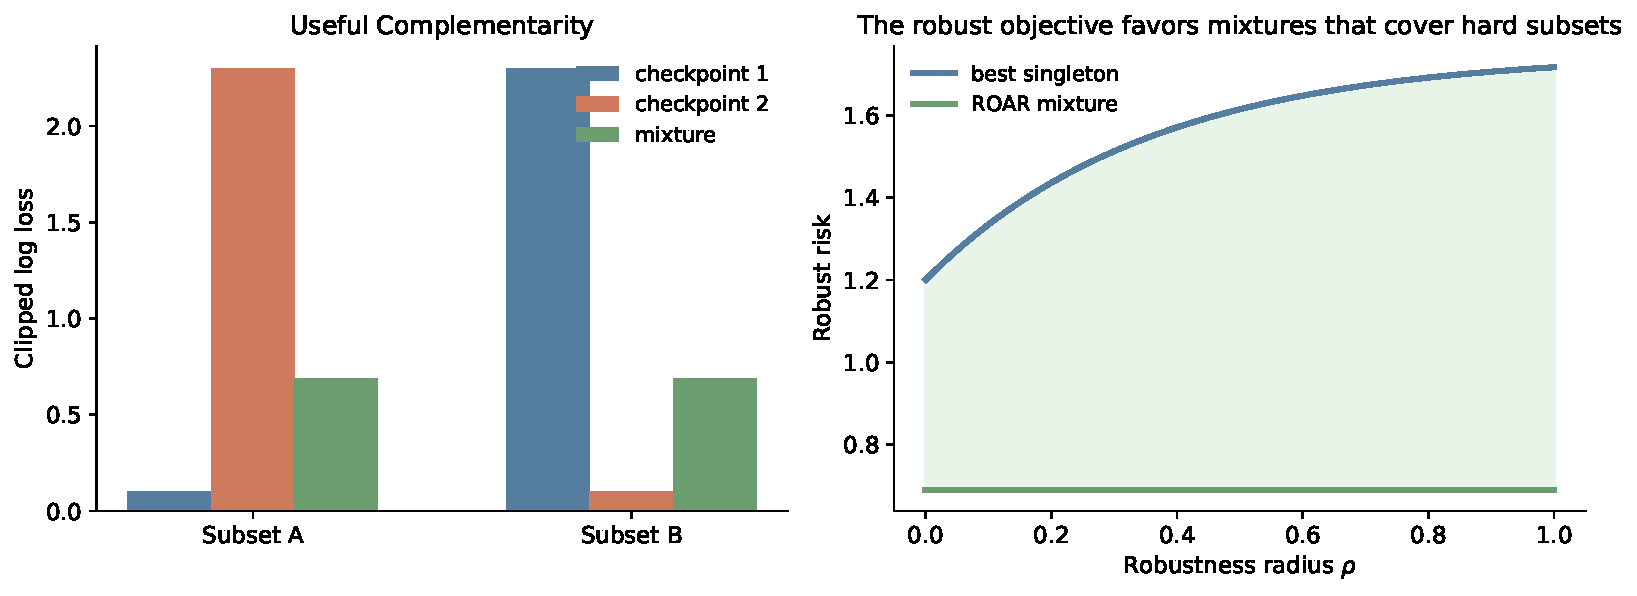
\includegraphics[width=\linewidth]{figures/safe_complementarity.pdf}
    \caption{A toy complementarity regime where every singleton checkpoint fails on one hard subset, while the mixture equalizes the losses and achieves a strictly smaller robust objective for every $\rho>0$. This is the exact phenomenon formalized in Proposition~\ref{prop:complementarity}.}
    \label{fig:complementarity}
\end{figure}

\subsection{Optimization guarantee}

\begin{theorem}[Projected subgradient convergence]
\label{thm:convergence}
Assume we run projected subgradient descent on $\mathcal U_{\rho}$ over the simplex with step sizes
\[
    \alpha_k = \frac{D}{G\sqrt{T}},
\]
where $D$ bounds the simplex diameter and $G$ is a uniform bound on the subgradient norm. Then the averaged iterate $\bar w_T=\frac{1}{T}\sum_{k=1}^{T} w^{(k)}$ satisfies
\begin{equation}
    \mathcal U_{\rho}(\bar w_T) - \mathcal U_{\rho}(w^{\star})
    \le
    \frac{DG}{\sqrt{T}}.
    \label{eq:subgrad_rate}
\end{equation}
With the clipping rule in Eq.~\eqref{eq:qit}, one may take
\[
    G \le \frac{\sqrt{|\cC|}}{\varepsilon_p}.
    \]
\end{theorem}

\subsection{From predictive mixture to deployed soup}

\begin{assumption}[Local second-order linearity]
\label{ass:locality}
For every feasible $w$ and every validation example $(x_i,y_i)$, define the true-class probability of the deployed weight soup by
\[
    \widetilde q_i(w) \triangleq p_{\theta(w)}(x_i)_{y_i},
    \qquad
    \theta(w)=\sum_{t\in\cC} w_t\theta_t.
    \]
Assume there exists a constant $\Gamma>0$ such that
\begin{equation}
    |\widetilde q_i(w)-\sum_{t\in\cC} w_t q_{it}|
    \le
    \Gamma \Delta(w)^2,
    \qquad
    \Delta(w)\triangleq \max_{t:w_t>0}\norm{\theta_t-\theta(w)}_2,
    \label{eq:locality_assumption}
\end{equation}
and $\widetilde q_i(w)\ge \varepsilon_p/2$ for all $i$.
\end{assumption}

Define the clipped deployed-soup loss and target risk by
\begin{equation}
    \ell^{\mathrm{soup}}((x,y);w)
    \triangleq
    -\log\!\Big(\max\{p_{\theta(w)}(x)_y,\varepsilon_p/2\}\Big),
    \qquad
    R_T^{\mathrm{soup}}(w)
    \triangleq
    \EE_{(x,y)\sim P_T}\big[\ell^{\mathrm{soup}}((x,y);w)\big].
    \label{eq:soup_loss_def}
\end{equation}

\begin{theorem}[Soup-transfer certificate]
\label{thm:soup_transfer}
Under Assumption~\ref{ass:locality}, the clipped loss of the deployed weight soup differs from the optimized predictive-mixture loss by at most
\begin{equation}
    \left|
        -\log \widetilde q_i(w)
        +
        \log\!\Big(\sum_{t\in\cC} w_t q_{it}\Big)
    \right|
    \le
    \frac{2\Gamma}{\varepsilon_p}\Delta(w)^2.
    \label{eq:loss_gap}
\end{equation}
Consequently,
\begin{equation}
    R_T^{\mathrm{soup}}(w)
    \le
    \mathcal U_{\rho}(w)
    +
    \frac{2\Gamma}{\varepsilon_p}\Delta(w)^2
    +
    \alpha \log(2/\varepsilon_p)
    \label{eq:soup_certificate}
\end{equation}
under Assumption~\ref{ass:support}.
\end{theorem}

This theorem is where approximate averageability enters the theory. It is the only approximation step between the exact objective and the final deployed model. Unlike \swad{}, the main selection objective is still optimized exactly; the locality assumption only transfers the optimized certificate to the final soup.

\section{Experimental Protocol and Published Baselines}
\label{sec:experiments}

\paragraph{Protocol.}
The intended evaluation protocol for \roar{} is the standard DomainBed ResNet-50 setting with dense checkpoints and pooled source-validation model selection \citep{gulrajani2021domainbed,cha2021swad}. \roar{} itself requires only a single training trajectory and a pooled labeled source-validation set. It does not require domain labels, test-time ensembling, or retraining.

\paragraph{Published baselines.}
Table~\ref{tab:single_run} reports exact published single-run post-hoc baselines from \swad{} and the closely related moving-average baseline reproduced by \diwa{}. Table~\ref{tab:frontier} reports broader published frontier numbers from \swad{}, \diwa{}, and \miro{}. These are not all identical protocols, so they should be interpreted as context rather than as a strict apples-to-apples leaderboard. All new \roar{} entries are intentionally left as \TBD{} until experiments are run.

\begin{table}[t]
    \centering
    \small
    \caption{\textbf{Published single-run post-hoc baselines on DomainBed ResNet-50.} Exact numbers reproduced from the published tables in \swad{} and \diwa{}. These are the most directly comparable baselines for \roar{}'s intended regime.}
    \label{tab:single_run}
    \begin{tabular}{lccccc|c}
        \toprule
        Algorithm & PACS & VLCS & OfficeHome & TerraInc & DomainNet & Avg. \\
        \midrule
        ERM \citep{cha2021swad} & 85.5 & 77.5 & 66.5 & 46.1 & 40.9 & 63.3 \\
        ERM + SWA$_{\text{const}}$ \citep{cha2021swad} & 86.9 & 76.6 & 69.3 & 49.2 & 45.9 & 65.6 \\
        MA \citep{rame2022diwa} & 87.5 & 78.2 & 70.6 & 50.3 & 46.0 & 66.5 \\
        \swad{} \citep{cha2021swad} & 88.1 & 79.1 & 70.6 & 50.0 & 46.5 & 66.9 \\
        \roar{} (ours) & \TBD{} & \TBD{} & \TBD{} & \TBD{} & \TBD{} & \TBD{} \\
        \bottomrule
    \end{tabular}
\end{table}

\begin{table}[t]
    \centering
    \small
    \caption{\textbf{Broader published frontier context.} These methods are informative reference points but not fully identical protocols. \diwa{} uses multi-run diversity and, in its strongest published setting, LP initialization. \miro{} is not a post-hoc soup method, but it is a strong DG baseline and combines well with \swad{}.}
    \label{tab:frontier}
    \begin{tabular}{lcc}
        \toprule
        Method & Setting & Published average \ood{} accuracy \\
        \midrule
        \swad{} \citep{cha2021swad} & single-run, ResNet-50 & 66.9 \\
        \diwa{} \citep{rame2022diwa} & multi-run, random init & 67.1 \\
        \diwa{}$^{\dagger}$ \citep{rame2022diwa} & multi-run, LP init & 68.0 \\
        \miro{} \citep{cha2022miro} & training-time DG method & 65.9 \\
        \miro{} + \swad{} \citep{cha2022miro} & training-time + post-hoc & 68.1 \\
        \roar{} (ours) & single-run, label-free post-hoc & \TBD{} \\
        \bottomrule
    \end{tabular}
\end{table}

\paragraph{What the new results section must test.}
The decisive empirical tests are:
\begin{enumerate}[leftmargin=1.4em]
    \item checkpoint-level correlation between $\mathcal U_{\rho}(w)$ and target \ood{} accuracy,
    \item head-to-head comparison against ERM, moving average, \swad{}, and any replayable \dcola{}-style selector on identical checkpoint trajectories,
    \item ablations over $\rho$, the barrier tolerance $\tau$, and the loss tolerance $\epsilon$,
    \item analysis of whether \roar{} finds nontrivial nonuniform soups rather than collapsing to a singleton,
    \item verification that improvements do not vanish when moving from the optimized predictive mixture to the actual deployed weight soup.
\end{enumerate}

\paragraph{Placeholder for results.}
\TBD{} We will insert the complete new results section here after running DomainBed-style experiments. This will include main tables, confidence intervals, checkpoint-level correlation plots, ablation tables, and diagnostics on soup sparsity and robustness radius.

\section{Discussion}

\paragraph{What \roar{} fixes relative to \swad{}.}
The main improvement is not just a stronger empirical prior. It is a better theory-to-algorithm alignment. \swad{} proves a robust-risk story and then deploys a valley heuristic. \roar{} directly optimizes the robust objective that its theory cares about. If the assumptions behind Theorem~\ref{thm:certificate} are accepted, there is no additional heuristic gap in the selector itself.

\paragraph{What \roar{} fixes relative to consensus-only methods.}
The robust objective does not ask for generic checkpoint agreement. It asks for coverage of hard but plausible reweightings. This is why \roar{} is a better synthesis of what worked in \swad{} and what worked in the more complementary soup behavior seen in \dcola{}-style experiments: useful disagreement is kept when it reduces robust risk and discarded when it is redundant or unsafe.

\paragraph{Limitations.}
The certificate is only as good as its shift model. Assumption~\ref{ass:support} says the unseen target is close to a reweighting of the observed source support, up to an explicit residual mass $\alpha$. That is a meaningful label-free assumption, but it is not universal. The soup-transfer theorem also depends on a locality condition similar in spirit to the assumptions behind weight averaging more broadly. Finally, \roar{} still requires dense checkpoints, which can increase storage costs.

\paragraph{Why this is still worth doing.}
Those limitations are honest and explicit, which is the point. The method is not justified by folklore; it is justified by a theorem whose assumptions are stated and whose optimized quantity is exactly the deployed selector's objective.

\section{Conclusion}

This paper proposed \roar{}, a label-free single-run post-hoc DG method built around one strict design principle: the algorithm should directly optimize the theoretical object it claims to improve. \roar{} does that by minimizing an exact KL-ball robust risk over simplex weights on a barrier-filtered candidate set of checkpoints from one training trajectory. The result is a method that is simple to state, convex to optimize, honest about its assumptions, and provably no worse on its own certificate than any feasible \swad{}-style interval or singleton checkpoint. If the next stage of DG research is to move beyond theory-motivated heuristics and toward theory-aligned post-hoc selectors, \roar{} is a concrete proposal for what that could look like.

\appendix

\section{Additional Visual Intuition}

\begin{figure}[H]
    \centering
    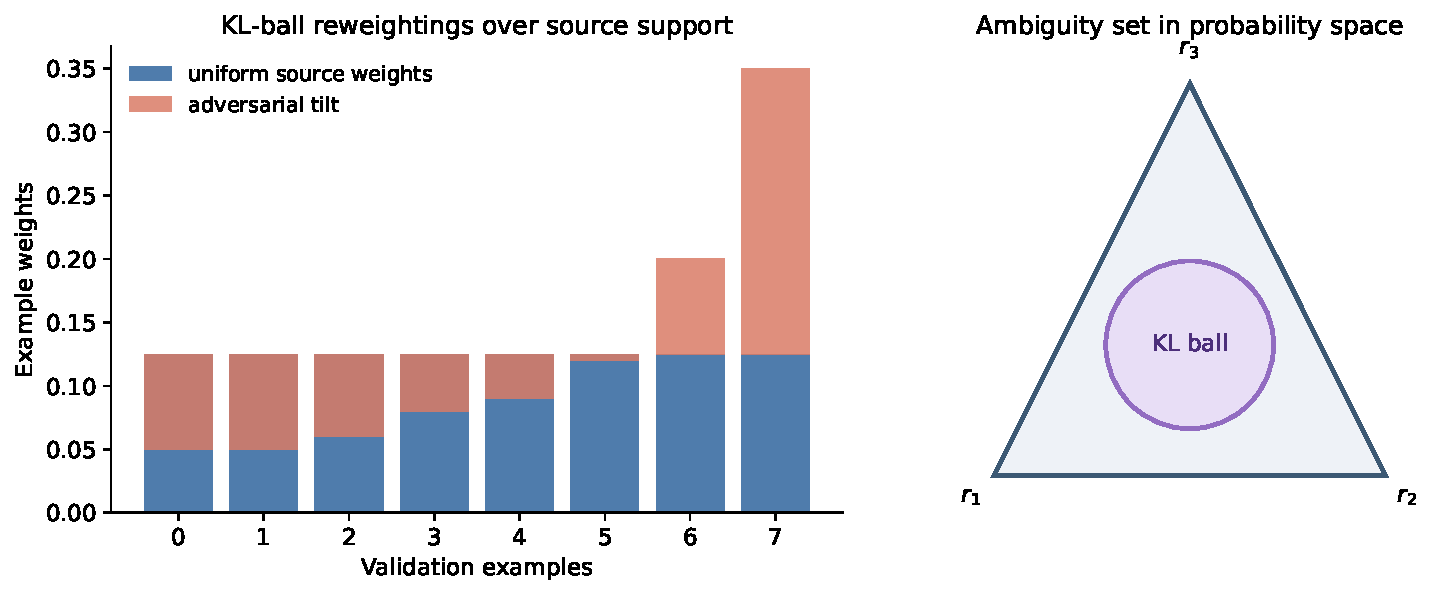
\includegraphics[width=0.82\linewidth]{figures/uncertainty_set.pdf}
    \caption{Visual intuition for the KL ambiguity set used by \roar{}. Left: example reweightings on a finite support. Right: a probability-simplex sketch of the ambiguity region.}
    \label{fig:uncertainty}
\end{figure}

\begin{figure}[H]
    \centering
    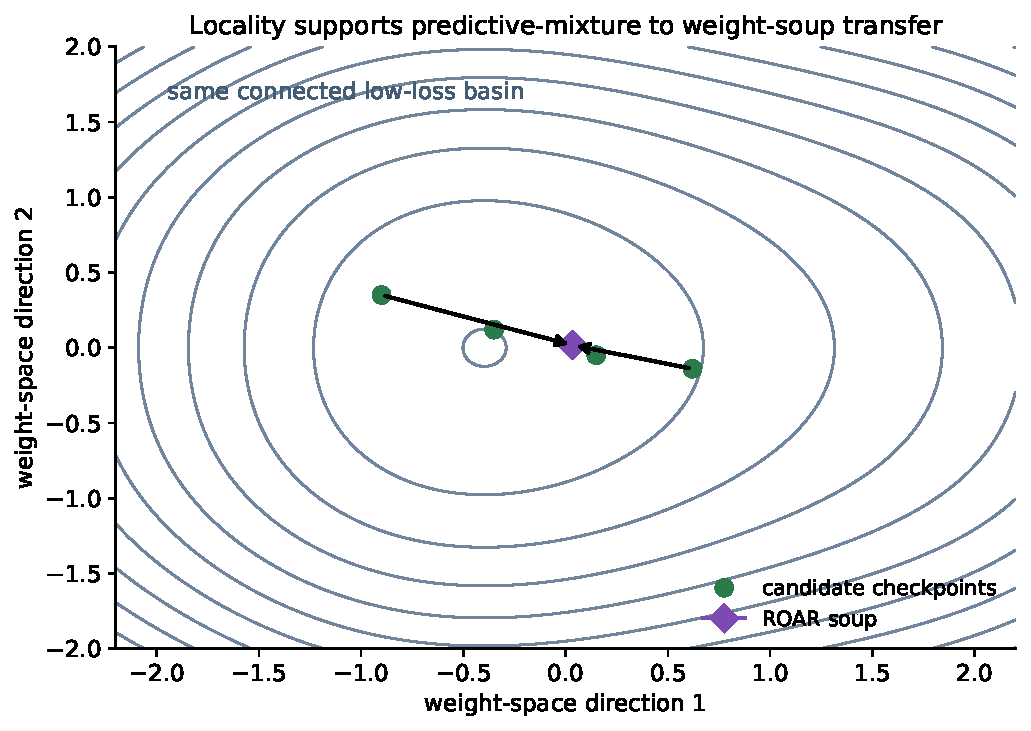
\includegraphics[width=0.8\linewidth]{figures/soup_transfer.pdf}
    \caption{Local second-order linearity intuition: when candidate checkpoints live inside one connected low-loss basin, the predictive mixture and the deployed weight soup are close enough for Theorem~\ref{thm:soup_transfer} to transfer the certificate.}
    \label{fig:soup_transfer}
\end{figure}

\section{Proof of Theorem~\ref{thm:dual}}

\begin{proof}
Fix $w$ and write $\ell_i=\ell_i(w)$ for brevity. The primal problem is
\[
    \sup_{r\in\RR^n}
    \left\{
        \sum_{i=1}^{n} r_i\ell_i
        :
        r_i\ge 0,\;
        \sum_{i=1}^{n} r_i = 1,\;
        \sum_{i=1}^{n} r_i \log(n r_i)\le \rho
    \right\}.
\]
Introduce a Lagrange multiplier $\eta\ge 0$ for the KL constraint and $\lambda\in\RR$ for the simplex-sum constraint. The Lagrangian is
\[
    \mathcal L(r,\eta,\lambda)
    =
    \sum_{i=1}^{n} r_i\ell_i
    -
    \eta\left(\sum_{i=1}^{n} r_i\log(n r_i)-\rho\right)
    -
    \lambda\left(\sum_{i=1}^{n} r_i-1\right).
\]
For $\eta>0$, maximizing $\mathcal L$ over $r_i\ge 0$ is separable. Differentiating with respect to $r_i$ gives
\[
    \ell_i - \eta(\log(nr_i)+1) - \lambda = 0,
\]
so
\[
    r_i
    =
    \frac{1}{n}\exp\!\left(\frac{\ell_i-\lambda-\eta}{\eta}\right).
\]
Imposing $\sum_i r_i=1$ yields
\[
    r_i
    =
    \frac{\exp(\ell_i/\eta)}{\sum_{j=1}^{n}\exp(\ell_j/\eta)}.
\]
Substituting this optimizer back into the Lagrangian gives the dual objective
\[
    \eta \rho + \eta \log\!\left(\frac{1}{n}\sum_{i=1}^{n}\exp(\ell_i/\eta)\right).
\]
By standard convex duality for finite-dimensional entropy-constrained maximization, strong duality holds, which proves Eq.~\eqref{eq:dual}. The formula for $r^{\star}$ is exactly the optimizer derived above.
\end{proof}

\section{Proof of Proposition~\ref{prop:limits}}

\begin{proof}
Let
\[
    K_w(t)
    \triangleq
    \log\!\left(\frac{1}{n}\sum_{i=1}^{n}\e^{t\ell_i(w)}\right)
\]
be the empirical cumulant-generating function of the clipped losses. Write $\bar \ell=\bar \ell(w)$ and $v=\operatorname{Var}_{u_n}(\ell(w))$. Then
\[
    K_w(t)= \bar \ell\, t + \frac{v}{2}t^2 + O(t^3)
    \qquad \text{as } t\downarrow 0.
\]
Setting $t=1/\eta$, the dual objective becomes
\[
    \eta\rho + \eta K_w(1/\eta)
    =
    \bar \ell + \eta\rho + \frac{v}{2\eta} + O(\eta^{-2}).
\]
Minimizing the leading nonconstant terms in $\eta$ gives
\[
    \eta^{\star}
    =
    \sqrt{\frac{v}{2\rho}} + O(1),
\]
and therefore
\[
    \mathcal U_{\rho}(w)
    =
    \bar \ell + \sqrt{2\rho\,v} + O(\rho).
\]
This proves part (i).

For part (ii), observe from Eq.~\eqref{eq:dual} that
\[
    \mathcal U_{\rho}(w)
    =
    \inf_{\eta>0}
    \left\{
        \eta\rho
        +
        \eta\log\!\left(\frac{1}{n}\sum_i \e^{\ell_i/\eta}\right)
    \right\}.
\]
For every fixed loss vector,
\[
    \lim_{\eta\downarrow 0}
    \eta\log\!\left(\sum_i \e^{\ell_i/\eta}\right)
    =
    \max_i \ell_i.
\]
As $\rho\to\infty$, the optimizer pushes toward the hard-subset regime, and the entropic risk tends to the maximum loss. This is the standard softmax-to-maximum limit, giving
\[
    \lim_{\rho\to\infty}\mathcal U_{\rho}(w)=\max_i \ell_i(w).
\]
\end{proof}

\section{Proof of Theorem~\ref{thm:convexity}}

\begin{proof}
For each $i$, the map
\[
    w\mapsto \sum_{t\in\cC} w_t q_{it}
\]
is affine and strictly positive on the simplex because $q_{it}\ge \varepsilon_p>0$. Since $x\mapsto -\log x$ is convex on $(0,\infty)$, each $\ell_i(w)$ is convex and continuous. For each fixed $r\in\cR_{\rho}$, the map
\[
    w\mapsto \sum_{i=1}^{n} r_i \ell_i(w)
\]
is a convex combination of convex continuous functions and is therefore convex and continuous. Equation~\eqref{eq:roar_primal} defines $\mathcal U_{\rho}$ as the supremum of these convex continuous functions over the nonempty set $\cR_{\rho}$, so $\mathcal U_{\rho}$ is convex and lower semicontinuous. Because every $\ell_i$ is bounded between $0$ and $L_{\max}$, the supremum is finite everywhere, hence $\mathcal U_{\rho}$ is continuous on the compact simplex. By the Weierstrass theorem, $\mathcal U_{\rho}$ attains its minimum on the simplex.
\end{proof}

\section{Proof of Theorem~\ref{thm:certificate}}

\begin{proof}
Under Assumption~\ref{ass:support}, write the target risk of the predictive mixture as
\[
    R_T^{\mathrm{mix}}(w)
    =
    (1-\alpha)\EE_{P_{\parallel}}[\ell(w)]
    +
    \alpha \EE_{P_{\perp}}[\ell(w)].
\]
Because $P_{\parallel}$ is supported on the validation examples and its density ratio relative to $\widehat P_{\cV}$ belongs to $\cR_{\rho}$, there exists $r\in\cR_{\rho}$ such that
\[
    \EE_{P_{\parallel}}[\ell(w)] = \sum_{i=1}^{n} r_i \ell_i(w) \le \mathcal U_{\rho}(w).
\]
Also, by clipping, $0\le \ell(w)\le L_{\max}$ everywhere, so
\[
    \EE_{P_{\perp}}[\ell(w)] \le L_{\max}.
\]
Combining the two inequalities gives
\[
    R_T^{\mathrm{mix}}(w)
    \le
    (1-\alpha)\mathcal U_{\rho}(w) + \alpha L_{\max}
    \le
    \mathcal U_{\rho}(w) + \alpha L_{\max}.
\]
If $\alpha=0$, the residual term vanishes and the exact certificate follows.
\end{proof}

\section{Proof of Theorem~\ref{thm:domination}}

\begin{proof}
The minimizer $w^{\star}$ solves
\[
    \mathcal U_{\rho}(w^{\star})
    =
    \min_{w\in\simplex^{|\cC|-1}} \mathcal U_{\rho}(w).
\]
Every feasible selector family $\mathfrak S$ in Definition~\ref{def:families} satisfies $\mathfrak S\subseteq \simplex^{|\cC|-1}$. Therefore
\[
    \mathcal U_{\rho}(w^{\star})
    \le
    \min_{w\in\mathfrak S}\mathcal U_{\rho}(w).
\]
This proves Eq.~\eqref{eq:domination}. The special cases for singleton checkpoints and contiguous uniform intervals are immediate by choosing $\mathfrak S=\mathfrak S_{\mathrm{single}}$ and $\mathfrak S=\mathfrak S_{\mathrm{int}}$.

Under Assumption~\ref{ass:support}, Theorem~\ref{thm:certificate} yields
\[
    R_T^{\mathrm{mix}}(w)
    \le
    \mathcal U_{\rho}(w) + \alpha L_{\max}
\]
for every feasible $w$. Applying this inequality at $w^{\star}$ and at any $w\in\mathfrak S$, then using the domination of $\mathcal U_{\rho}(w^{\star})$, transfers the no-worse guarantee to the certified target-risk upper bound.
\end{proof}

\section{Proof of Proposition~\ref{prop:complementarity}}

\begin{proof}
Define
\[
    a=-\log(1-\delta), \qquad b=-\log(\delta).
\]
For checkpoint $e_1$, the losses equal $a$ on $A$ and $b$ on $B$. For checkpoint $e_2$, the pattern is reversed. For the equal mixture,
\[
    \sum_{t=1}^{2} w_t^{\mathrm{mix}} q_{it}
    =
    \frac{(1-\delta)+\delta}{2}
    =
    \frac{1}{2}
\]
for every example, so
\[
    \ell_i(w^{\mathrm{mix}})=\log 2
    \qquad \text{for all } i.
\]
Hence the robust objective of the mixture is constant:
\[
    \mathcal U_{\rho}(w^{\mathrm{mix}})=\log 2.
\]

Now consider a singleton checkpoint, say $e_1$. Its loss vector is nonconstant with half the examples at $a$ and half at $b$. Since $\rho>0$, the uniform weighting $u_n$ belongs to $\cR_{\rho}$. Therefore the primal robust objective is bounded below by the ordinary empirical mean:
\[
    \mathcal U_{\rho}(e_1)
    \ge
    \frac{a+b}{2}.
\]
Since $\delta(1-\delta)<1/4$ for every $0<\delta<1/2$,
\[
    \frac{a+b}{2}
    =
    -\frac{1}{2}\log(\delta(1-\delta))
    >
    -\frac{1}{2}\log(1/4)
    =
    \log 2.
\]
Combining the inequalities gives
\[
    \mathcal U_{\rho}(w^{\mathrm{mix}})
    =
    \log 2
    <
    \mathcal U_{\rho}(e_1).
\]
By symmetry, $\mathcal U_{\rho}(e_1)=\mathcal U_{\rho}(e_2)$, proving the claim.
\end{proof}

\section{Proof of Theorem~\ref{thm:convergence}}

\begin{proof}
This is the standard projected subgradient bound. Let $w^{(k+1)}=\Pi_{\simplex}(w^{(k)}-\alpha_k g^{(k)})$ where $g^{(k)}\in \partial \mathcal U_{\rho}(w^{(k)})$ and $\norm{g^{(k)}}_2\le G$. Nonexpansiveness of Euclidean projection gives, for any minimizer $w^{\star}$,
\[
    \norm{w^{(k+1)}-w^{\star}}_2^2
    \le
    \norm{w^{(k)}-\alpha_k g^{(k)}-w^{\star}}_2^2.
\]
Expanding the right-hand side,
\[
    \norm{w^{(k+1)}-w^{\star}}_2^2
    \le
    \norm{w^{(k)}-w^{\star}}_2^2
    -2\alpha_k \inner{g^{(k)}}{w^{(k)}-w^{\star}}
    + \alpha_k^2 \norm{g^{(k)}}_2^2.
\]
By the subgradient inequality,
\[
    \mathcal U_{\rho}(w^{(k)})-\mathcal U_{\rho}(w^{\star})
    \le
    \inner{g^{(k)}}{w^{(k)}-w^{\star}}.
\]
Substituting and summing from $k=1$ to $T$ yields
\[
    2\sum_{k=1}^{T}\alpha_k\big(\mathcal U_{\rho}(w^{(k)})-\mathcal U_{\rho}(w^{\star})\big)
    \le
    \norm{w^{(1)}-w^{\star}}_2^2
    + \sum_{k=1}^{T}\alpha_k^2 G^2.
\]
With the constant step size $\alpha_k = D/(G\sqrt{T})$ and simplex diameter bounded by $D$, Jensen's inequality gives the averaged-iterate bound
\[
    \mathcal U_{\rho}(\bar w_T)-\mathcal U_{\rho}(w^{\star})
    \le
    \frac{DG}{\sqrt{T}}.
\]

It remains to justify the gradient bound. From Eq.~\eqref{eq:gradient},
\[
    \left|\big(\nabla \mathcal U_{\rho}(w)\big)_t\right|
    \le
    \sum_{i=1}^{n} r_i^{\star}(w)\frac{q_{it}}{s_i(w)}
    \le
    \sum_{i=1}^{n} r_i^{\star}(w)\frac{1}{\varepsilon_p}
    =
    \frac{1}{\varepsilon_p}.
\]
Hence
\[
    \norm{\nabla \mathcal U_{\rho}(w)}_2
    \le
    \frac{\sqrt{|\cC|}}{\varepsilon_p}.
\]
\end{proof}

\section{Proof of Theorem~\ref{thm:soup_transfer}}

\begin{proof}
Fix a feasible $w$ and an index $i$. Let
\[
    s_i(w)=\sum_{t\in\cC} w_t q_{it}.
\]
By Assumption~\ref{ass:locality},
\[
    |\widetilde q_i(w)-s_i(w)|
    \le
    \Gamma \Delta(w)^2.
\]
Also, $s_i(w)\ge \varepsilon_p$ and $\widetilde q_i(w)\ge \varepsilon_p/2$. The derivative of $x\mapsto -\log x$ on $[\varepsilon_p/2,1]$ is bounded in magnitude by $2/\varepsilon_p$. Therefore, by the mean value theorem,
\[
    \left|
        -\log \widetilde q_i(w) + \log s_i(w)
    \right|
    \le
    \frac{2}{\varepsilon_p} |\widetilde q_i(w)-s_i(w)|
    \le
    \frac{2\Gamma}{\varepsilon_p}\Delta(w)^2.
\]
This proves Eq.~\eqref{eq:loss_gap}.

Define the clipped loss of the deployed soup on example $i$ by
\[
    \widetilde \ell_i(w) = -\log \widetilde q_i(w).
\]
The pointwise bound above implies
\[
    \widetilde \ell_i(w)
    \le
    \ell_i(w) + \frac{2\Gamma}{\varepsilon_p}\Delta(w)^2
    \qquad \text{for all } i.
\]
Taking the supremum over $r\in\cR_{\rho}$ preserves this additive constant:
\[
    \sup_{r\in\cR_{\rho}}\sum_i r_i \widetilde \ell_i(w)
    \le
    \mathcal U_{\rho}(w) + \frac{2\Gamma}{\varepsilon_p}\Delta(w)^2.
\]
Applying Theorem~\ref{thm:certificate} to the deployed soup losses yields
\[
    R_T^{\mathrm{soup}}(w)
    \le
    \mathcal U_{\rho}(w)
    +
    \frac{2\Gamma}{\varepsilon_p}\Delta(w)^2
    +
    \alpha \log(2/\varepsilon_p),
\]
which is Eq.~\eqref{eq:soup_certificate}.
\end{proof}

\section{Implementation Notes}

\paragraph{Why clipping is part of the method.}
The clipping in Eq.~\eqref{eq:qit} is not cosmetic. It is what makes the losses bounded, the subgradients controlled, and the support-mismatch term in Theorem~\ref{thm:certificate} finite. In practice $\varepsilon_p$ should be set very small, but not zero.

\paragraph{Why the barrier is still needed.}
The robust objective is the exact theoretical object, but the deployment target is still a \emph{weight soup}. The candidate filter is therefore not an extra heuristic objective term; it is the feasible-set definition that makes Theorem~\ref{thm:soup_transfer} plausible. This is a narrower and more defensible role than in prior flatness-window methods.

\paragraph{What remains empirical.}
The only irreducibly empirical parts of the method are the hyperparameters $(\epsilon,\tau,\rho,\varepsilon_p)$ and the practical barrier computation. The selector itself is not heuristic once those are fixed; it is the exact optimizer of Eq.~\eqref{eq:roar_primal}.

\bibliographystyle{plainnat}
\bibliography{references}

\end{document}
